\documentclass[letterpaper]{article}
\usepackage[submission]{aaai2027}
\usepackage[hyphens]{url}
\usepackage{graphicx}
\urlstyle{rm}
\def\UrlFont{\rm}
\usepackage{natbib}
\usepackage{caption}
\frenchspacing

\pdfinfo{
/TemplateVersion (2027.1)
}

\usepackage{amsmath}
\usepackage{amssymb}
\usepackage{booktabs}
\usepackage{multirow}
\usepackage{array}
\usepackage{tabularx}
\usepackage{enumitem}
\usepackage{xspace}
\usepackage{tikz}
\usetikzlibrary{shapes.geometric,arrows,positioning,calc,fit}
\newcolumntype{Y}{>{\raggedright\arraybackslash}X}

\newcommand{\method}{MemPatch}
\newcommand{\bench}{MemPatch-Bench}
\newcommand{\rmi}{Rapid Memory Integration}
\newcommand{\rmiabbr}{RMI}
\newcommand{\dpafull}{Revision Guard}
\newcommand{\dpa}{\dpafull{}}
\newcommand{\pathfull}{\method{}}
\newcommand{\pathnodpa}{Typed Revision Scaffold}
\newcommand{\pathdirect}{Direct State Prediction}
\newcommand{\field}[1]{\textit{#1}}
\newcommand{\fname}[1]{{\fontfamily{phv}\selectfont\small #1}}
\newcommand{\state}{\field{memory\_state}}
\newcommand{\decision}{\field{decision}}
\newcommand{\evidence}{\field{evidence\_event\_ids}}
\newcommand{\diagnosis}{\field{failure\_diagnosis}}
\newcommand{\answer}{\field{answer}}
\newcommand{\joint}{joint revision success}

\title{MemPatch: Evidential Revision Scaffolds for Rapid Memory Integration in LLM Agents}
\author{Anonymous Submission}
\affiliations{}

\begin{document}
\maketitle

\begin{abstract}
Persistent-memory large language model (LLM) agents use stored records to guide future retrieval and action, yet corrective evidence can invalidate a record without removing its license for downstream reuse. Answer accuracy alone can therefore hide a corrupted persistent state. We introduce \bench{}, a benchmark for post-admission memory revision with executable reference semantics, record-level validity labels, and a development-calibrated diagnostic profile. We also introduce \method{}, a parameter-free mediation layer that compiles model proposals into typed patches, checks them against a deterministic Revision Guard, and emits a replayable commit certificate. Under matched frozen backbones, canonical projection yields $100\%$ final-response schema compliance while raw action parse validity ranges from $87.8\%$ to $100\%$. \method{} also stabilizes memory-state prediction, including $84.7\%$ state accuracy on a backbone whose strongest frozen baseline reaches $9.3\%$. The gains are not uniform across every answer-level metric: structured mediation can trade proposal recall for state integrity. We separate guarantees of the deterministic mediator from empirical properties of the neural proposer, yielding an evaluation and runtime framework for memory updates that are explicit, evidence-grounded, and externally auditable.

\end{abstract}

\section{Introduction}

Large language model (LLM) agents are increasingly deployed in long-horizon environments where they must maintain state across extended temporal trajectories. Rather than relying solely on transient context windows, modern agent architectures employ persistent memory stores to accumulate experiences, document tool executions, and record intermediate planning states. These stored records actively guide subsequent system behaviors, serving as the knowledge base for downstream retrieval, planning, tool use, and database writes. In this persistent setting, a critical and under-addressed risk is record obsolescence—where a persistent record remains licensed for future reuse after corrective, conflicting, superseding, or policy-relevant evidence has arrived. 

Retrieval alone does not solve this problem. For example, a calendar agent may persistently store that a user has a meeting scheduled on Tuesday. When subsequent email evidence reveals that the meeting has been moved to Friday, the agent must update its memory state. If the agent retrieves the new email and answers the immediate query correctly while leaving the contradicted Tuesday record active in its store, subsequent tasks may retrieve the stale Tuesday record, leading to scheduling conflicts. This silent failure permits immediate query success but leaves a contaminated state that propagates errors in future execution turns.

\begin{figure*}[t]
\centering
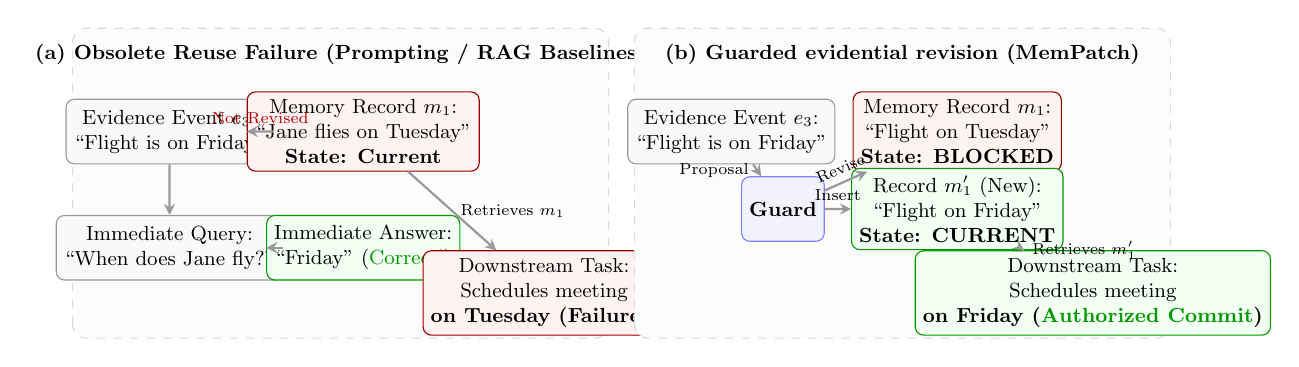
\begin{tikzpicture}[
    scale=0.82, every node/.style={transform shape},
    box/.style={rectangle, draw=gray!80, fill=gray!5, rounded corners=3pt, minimum width=2.4cm, minimum height=1.0cm, align=center, font=\small},
    greenbox/.style={rectangle, draw=green!60!black, fill=green!5, rounded corners=3pt, minimum width=2.4cm, minimum height=1.0cm, align=center, font=\small},
    redbox/.style={rectangle, draw=red!60!black, fill=red!5, rounded corners=3pt, minimum width=2.4cm, minimum height=1.0cm, align=center, font=\small},
    title/.style={font=\bfseries\small},
    arrow/.style={->, >=stealth, thick, draw=gray!80},
    dasharrow/.style={->, >=stealth, dashed, thick, draw=gray!80}
]

% PANEL A: Baseline
\draw[gray!30, fill=gray!2, dashed, rounded corners=5pt] (-0.5,-1.2) rectangle (7.8,3.6);
\node[title] at (3.65,3.2) {(a) Obsolete Reuse Failure (Prompting / RAG Baselines)};

\node[box] (eva) at (1.0,2.0) {Evidence Event $e_3$:\\``Flight is on Friday''};
\node[redbox] (mema) at (4.0,2.0) {Memory Record $m_1$:\\``Jane flies on Tuesday''\\\textbf{State: Current}};
\node[box] (querya) at (1.0,0.2) {Immediate Query:\\``When does Jane fly?''};
\node[greenbox] (ansa) at (4.0,0.2) {Immediate Answer:\\``Friday'' (\textcolor{green!60!black}{Correct!})};
\node[redbox] (downa) at (6.8,-0.5) {Downstream Task:\\Schedules meeting\\\textbf{on Tuesday (Failure!)}};

\draw[arrow] (eva) -- (mema) node[midway,above,font=\scriptsize,text=red!70!black] {Not Revised};
\draw[arrow] (eva) -- (querya);
\draw[arrow] (querya) -- (ansa);
\draw[arrow] (mema) -- (downa) node[midway,right,font=\scriptsize] {Retrieves $m_1$};

% PANEL B: MemPatch
\draw[gray!30, fill=gray!2, dashed, rounded corners=5pt] (8.2,-1.2) rectangle (16.5,3.6);
\node[title] at (12.35,3.2) {(b) Guarded evidential revision (MemPatch)};

\node[box] (evb) at (9.7,2.0) {Evidence Event $e_3$:\\``Flight is on Friday''};
\node[redbox] (membone) at (13.2,2.0) {Memory Record $m_1$:\\``Flight on Tuesday''\\\textbf{State: BLOCKED}};
\node[greenbox] (membtwo) at (13.2,0.8) {Record $m_{1}'$ (New):\\``Flight on Friday''\\\textbf{State: CURRENT}};

\node[box, minimum width=1.0cm, fill=blue!5, draw=blue!50] (guard) at (10.5,0.8) {\textbf{Guard}};

\node[greenbox] (downb) at (15.3,-0.5) {Downstream Task:\\Schedules meeting\\\textbf{on Friday (\textcolor{green!60!black}{Authorized Commit})}};

\draw[arrow] (evb) -- (guard) node[midway,left,font=\scriptsize] {Proposal};
\draw[arrow] (guard) -- (membone) node[midway,above,sloped,font=\scriptsize] {Revise};
\draw[arrow] (guard) -- (membtwo) node[midway,above,font=\scriptsize] {Insert};
\draw[arrow] (membtwo) -- (downb) node[midway,right,font=\scriptsize] {Retrieves $m_1'$};

\end{tikzpicture}
\caption{Comparison of memory integration mechanisms. (a) Traditional agent memory systems retrieve new evidence for immediate queries but leave obsolete records active in memory, causing downstream failures. (b) \method{} routes updates through a deterministic Guard and DPA kernel to revise memory states, preventing stale record reuse.}
\label{fig:motivation}
\end{figure*}

To isolate and evaluate this failure mode, we present \bench{}, a diagnostic benchmark specifically designed to evaluate post-admission validity revision in persistent agent memory. \bench{} requires agents to maintain record-level validity states under chronological evidence streams, scoring updates against hidden ground-truth labels. It evaluates agents not merely on their downstream answers, but on their ability to perform joint revision, scoring the concurrent correctness of task decisions, memory validity states, evidence citations, failure diagnoses, and answers. 

To address this challenge without parameter updates, we propose \method{}, a parameter-free plug-in runtime layer that separates opaque semantic proposals from verifiable persistent-memory transitions. \method{} does not expose the model's latent reasoning. It confines black-box inference to semantic proposal and makes every committed persistent-memory transition explicit, authorization-checked, and replayable. Specifically, \method{} queries a frozen backbone model through a dual-path proposal interface to obtain global states and local typed patches. These proposals are compiled into structured actions and routed through a deterministic, symbolic Revision Guard and a conservative reconciliation function before projecting to memory. 

Empirical evaluations of frozen backbones (Qwen, Gemma, Phi-4, Mistral) show that standard prompting, retrieval-augmented generation (RAG), and memory baselines suffer severe integration failures. By separating semantic proposal generation from deterministic verification, \method{} significantly reduces stale-record reuse and improves memory state consistency without requiring task-specific parameter updates.

This paper makes the following co-equal primary contributions:
\begin{enumerate}[leftmargin=*]
\item \textbf{\bench{}:} A controlled benchmark for evaluating post-admission validity revision. It features record-level validity states, chronological evidence tracking, failure diagnoses, and strict joint evaluation to detect stale memory reuse and integration errors.
\item \textbf{\method{}:} A parameter-free plug-in runtime layer that uses a dual-path proposer interface to separate black-box neural proposals from deterministic, authorization-checked, and replayable memory transitions.
\item \textbf{Empirical Characterization:} An evaluation of frozen models showing that while standard prompting and RAG baselines are vulnerable to stale memory reuse, \method{} consistently enforces safety invariants, reducing the externally unverifiable transition surface to zero.
\end{enumerate}

\section{Related Work}

\paragraph{Memory Storage, Admission, and Retrieval.}
Existing architectures focus on memory storage structures, retrieval models, and periodic summarization or compression. Works such as \fname{MemGPT} manage memory via paging and swapping between a context window and external storage \cite{packer_memgpt_2024}. \fname{Mem0} provides CRUD-like operations over natural-language facts \cite{chhikara_mem0_2025}, while systems like \fname{A-MEM} and \fname{MemoryOS} focus on hierarchical organization, node consolidation, and context length reduction \cite{xu_-mem_2025,kang_memory_2025}. More recent methods learn memory operation selection or adaptive structures \cite{yu_agentic_2026,lu_choosing_2026,xu_structmem_2026,zhang_adaptive_2026}. 
Unlike these frameworks which optimize storage allocation or retrieval performance, \bench{} and \method{} focus strictly on \emph{post-admission validity revision}—validating whether existing memory records remain logically active or superseded as new evidence chronologically arrives.

\paragraph{Memory Benchmarks.}
Standard evaluations assess long-term retrieval, QA over extended chat histories, or task success in evolving virtual environments. The \textsc{LoCoMo} benchmarks evaluate conversational memory recall over tens of thousands of tokens \cite{maharana_evaluating_2024,li_locomo-plus_2026}. The \textsc{LongMemEval} family assesses temporal updates and experience acquisition in dialogue systems \cite{wu_longmemeval_2025,wu_longmemeval-v2_2026}. Other benchmarks study memory structure or self-evolving retrieval performance \cite{tan_membench_2025,shutova_evaluating_2026,wang_evomembench_2026,hu_evaluating_2026}. 
In contrast to evaluating memory through downstream answer accuracy (which can mask invalid memory states), \bench{} scores the record-level validity mapping directly, tracking evidence grounding and multi-dimensional error metrics.

\paragraph{Structured Inference and Runtime Enforcement.}
Inference-time scaffolds structure language model reasoning without parameter updates. \fname{ReAct} interleaves reasoning and actions \cite{yao_react_2023}, while \fname{Reflexion} and \fname{Self-Refine} implement feedback loops for self-correction \cite{shinn_reflexion_2023,madaan_self-refine_2023}. Reasoning pathways are generalized into thoughts in \textsc{Tree of Thoughts} and \textsc{Graph of Thoughts} \cite{yao_tree_2023,besta_graph_2024,zhou_language_2024,luo_graph_2026}. Embodied agents like \fname{Voyager} execute neural code proposals within deterministic environment engines \cite{wang_voyager_2023}. 
\method{} builds on these paradigms by splitting opaque neural generation from deterministic, symbolic state updates. However, we apply this separation specifically to memory revision, routing neural proposals through a symbolic Guard to verify references and resolve conflicts.

\paragraph{Benchmark Validity and Metamorphic Testing.}
Evaluating the robustness of benchmark evaluations is critical to prevent metric contamination. Metamorphic testing validates system behavior under semantics-preserving transformations (e.g., identifier renaming, event permutation) to assert mathematical equivariance and identify shortcut-learning patterns in models. We employ these principles to audit our diagnostic channels and verify the correctness of the reference transition engine.

\section{Problem Formulation}

We formalize the problem of post-admission memory validity revision. Let a scenario be defined as a tuple:
\begin{equation}
x = (M, E, q, c),
\end{equation}
where $M=\{m_i\}_{i=1}^{n}$ is the persistent memory store, $E=\{e_j\}_{j=1}^{k}$ is the chronological evidence ledger, $q$ is the downstream query, and $c$ contains public policy and scope constraints. Both memory records and evidence events are associated with unique, stable identifiers and natural-language payloads.

The public revision view is constructed via a deterministic function $B$:
\begin{equation}
V = B(M, E, q, c, s^0, \Gamma),
\end{equation}
where $s^0$ is the initial state map of the memory records, and $\Gamma$ is the published transition policy. Crucially, $V$ excludes gold labels, private metadata, and evaluator-specific information, exposing only the candidate records, evidence ledger, and active policies to the agent.

The memory state space $\Sigma$ is defined over five distinct epistemic classes:
\begin{equation}
\begin{split}
\Sigma=\{&\mathsf{Current},\mathsf{Blocked},\mathsf{Unresolved},\\
&\mathsf{OutOfScope},\mathsf{ShouldNotStore}\}.
\end{split}
\end{equation}
The downstream reuse license is a function $\lambda: \Sigma \rightarrow \{0, 1\}$:
\begin{equation}
\lambda(z) = \mathbf{1}[z = \mathsf{Current}],
\end{equation}
which dictates that a memory record $m_i$ is licensed for future reuse in downstream tasks if and only if its validity state $s_i$ is $\mathsf{Current}$. Records with other states (e.g., blocked due to unmet dependencies, unresolved due to conflicting evidence, contextually out-of-scope, or excluded by safety policy) are restricted from reuse.

\paragraph{Output Contract.}
The agent's output is structured as a tuple:
\begin{equation}
r = (d, \mathbf{s}, Z, f, a),
\end{equation}
where $d$ is a downstream decision (e.g., use memory, escalate, ask clarification, refuse due to policy), $\mathbf{s}: M \rightarrow \Sigma$ is the final memory validity mapping, $Z \subseteq I_E$ is the response-level evidence set, $f \in \mathcal{F}$ is the failure diagnosis, and $a$ is the final generated answer. For a committed patch, provenance is finer grained: $\widehat Z:M\rightarrow 2^{I_E}$ associates each changed record with its own evidence witness.

\paragraph{Diagnostic Measurement Model.}
To assess agent performance without hiding failure modes inside a single conjunction, we define seven response channels: decision, state, evidence, minimality, diagnosis, answer, and schema. They correspond to decision accuracy, memory-state accuracy, evidence $F_1$, minimal-evidence exact match, diagnosis accuracy, answer key-fact accuracy, and schema compliance. We probe these channels with seven controlled corruptions $\mathcal{O}$: wrong decision, wrong state, wrong evidence, overcitation, wrong diagnosis, malformed schema, and missing answer. Trace audit is evaluated separately because replayability is a property of an executed transition, not of a five-field response.

For each scenario, we define an error vector $\mathbf{e}(r, g) = (\ell_k(r, g))_{k \in \mathcal{K}}$, where each $\ell_k$ measures the correctness of output channel $k$ against gold label $g$. The diagnostic profile of an agent $h$ is the expected error vector:
\begin{equation}
\mathbf{R}(h) = \mathbb{E}_{\xi} [\mathbf{e}(h(B(\xi)), g(\xi))].
\end{equation}
The sensitivity matrix $A=(a_{kj})\in\mathbb{R}^{7\times7}$ records the decrement in metric $k$ under corruption $o_j$. All operators, mappings, and calibration constants are fixed exclusively on the L3 development split before L4 evaluation. Full rank is an empirical audit of this chosen corruption basis, not a claim that all real model failures are linearly separable. We report the complete error vector as the primary outcome. Joint revision success, $J(\mathbf b)=\prod_k(1-b_k)$, is retained only as a secondary complete-case statistic because it maps many distinct error signatures to the same zero value.

\section{\bench{}}

We introduce \bench{}, a diagnostic evaluation suite for post-admission memory validity revision. Unlike existing evaluations that assess memory quality through downstream task success, \bench{} directly audits the record-level validity state of the agent's memory store.

\paragraph{Dataset Composition and Statistics.}
The dataset contains a total of $4,000$ scenarios:
\begin{itemize}[leftmargin=*]
\item \textbf{L3 Development Split ($3,500$ cases):} Designed for prompt engineering, schema validation, Guard testing, ablation development, controlled corruption generation, and future supervised training.
\item \textbf{L4 Held-Out Split ($500$ cases):} Disjoint in templates and domains from L3, serving as the sole official evaluation split.
\end{itemize}
The scenarios span six diverse domains (software engineering, task management, data analysis, enterprise tooling, customer support, and scientific work) and are structured using stable, semantic-free identifiers.

\begin{figure*}[t]
\centering
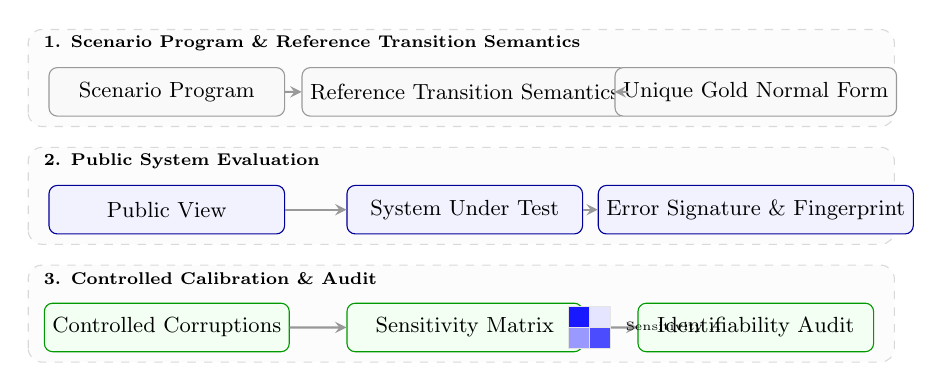
\begin{tikzpicture}[
    scale=0.88, every node/.style={transform shape},
    box/.style={rectangle, draw=gray!80, fill=gray!5, rounded corners=3pt, minimum width=3.4cm, minimum height=0.7cm, align=center, font=\small},
    bluebox/.style={rectangle, draw=blue!60!black, fill=blue!5, rounded corners=3pt, minimum width=3.4cm, minimum height=0.7cm, align=center, font=\small},
    greenbox/.style={rectangle, draw=green!60!black, fill=green!5, rounded corners=3pt, minimum width=3.4cm, minimum height=0.7cm, align=center, font=\small},
    arrow/.style={->, >=stealth, thick, draw=gray!80}
]

% Part 1: Gold Semantics
\draw[gray!30, fill=gray!2, dashed, rounded corners=5pt] (-0.5,1.2) rectangle (12.0,2.6);
\node[anchor=west, font=\bfseries\scriptsize] at (-0.4,2.4) {1. Scenario Program \& Reference Transition Semantics};
\node[box] (g1) at (1.5,1.7) {Scenario Program};
\node[box] (g2) at (5.8,1.7) {Reference Transition Semantics};
\node[box] (g3) at (10.0,1.7) {Unique Gold Normal Form};
\draw[arrow] (g1) -- (g2);
\draw[arrow] (g2) -- (g3);

% Part 2: System Evaluation
\draw[gray!30, fill=gray!2, dashed, rounded corners=5pt] (-0.5,-0.5) rectangle (12.0,0.9);
\node[anchor=west, font=\bfseries\scriptsize] at (-0.4,0.7) {2. Public System Evaluation};
\node[bluebox] (s1) at (1.5,0) {Public View};
\node[bluebox] (s2) at (5.8,0) {System Under Test};
\node[bluebox] (s3) at (10.0,0) {Error Signature \& Fingerprint};
\draw[arrow] (s1) -- (s2);
\draw[arrow] (s2) -- (s3);

% Part 3: Calibration & Audit
\draw[gray!30, fill=gray!2, dashed, rounded corners=5pt] (-0.5,-2.2) rectangle (12.0,-0.8);
\node[anchor=west, font=\bfseries\scriptsize] at (-0.4,-1.0) {3. Controlled Calibration \& Audit};
\node[greenbox] (c1) at (1.5,-1.7) {Controlled Corruptions};
\node[greenbox] (c2) at (5.8,-1.7) {Sensitivity Matrix};
\node[greenbox] (c3) at (10.0,-1.7) {Identifiability Audit};
\draw[arrow] (c1) -- (c2);
\draw[arrow] (c2) -- (c3);

% Small Heatmap inset in Part 3
\begin{scope}[shift={(7.3,-2.0)}]
    \draw[fill=blue!90, draw=gray!20] (0,0.3) rectangle (0.3,0.6);
    \draw[fill=blue!10, draw=gray!20] (0.3,0.3) rectangle (0.6,0.6);
    \draw[fill=blue!40, draw=gray!20] (0,0) rectangle (0.3,0.3);
    \draw[fill=blue!70, draw=gray!20] (0.3,0) rectangle (0.6,0.3);
    \node[right, font=\tiny] at (0.7,0.3) {Sensitivity $A$};
\end{scope}

\end{tikzpicture}
\caption{MemPatch-Bench evaluation protocol and diagnostic calibration pipeline. Raw programs yield a unique gold normal form under reference semantics. Agent outputs on public views produce multi-dimensional error signatures audited via controlled calibration.}
\label{fig:benchmark_pipeline}
\end{figure*}

\paragraph{Seven Memory Integration Failure Modes.}
Each scenario in \bench{} targets one of seven structural memory integration failures:
\begin{enumerate}[leftmargin=*]
\item \textbf{Stale-Reuse:} Obsolete records remain licensed for downstream reuse after contradictory evidence arrives.
\item \textbf{Under-Update:} Failure to identify and modify records targeted by valid updates.
\item \textbf{Conflict Collapse:} Concurrent contradictory updates leave the memory in an inconsistent, unresolved state without proper fail-closed logging.
\item \textbf{Scope Leakage:} Contextual or domain-specific exclusions are ignored, leaking out-of-scope records into active reasoning.
\item \textbf{Wrong-Source Attribution:} Crediting updates to incorrect or ungrounded evidence events.
\item \textbf{Policy Violation:} Violating safety, retention, or privacy constraints during memory modification.
\item \textbf{Memory Hallucination:} Proposing modifications to records that do not exist or using non-existent evidence identifiers.
\end{enumerate}

\paragraph{Evaluation Protocol.}
The evaluation protocol strictly isolates the hidden gold labels from the agent. The evaluator is fully deterministic, scoring output tuples $r = (d, \mathbf{s}, Z, f, a)$ to populate the diagnostic response matrix. Under Theorem~\ref{thm:gold_determinacy}, every valid scenario has a unique normal form determined by the transition rules, preventing shortcuts from masking state defects.

To enforce statistical rigor, \bench{} aggregates scenarios into hierarchical clusters defined by their underlying \emph{template family}. The L4 evaluation split comprises 500 instances partitioned into 18 unique template families, stratified across the seven failure modes: wrong source attribution (2 families, 75 instances), scope leakage (2 families, 75 instances), under-update (2 families, 87 instances), conflict collapse (6 families, 124 instances), policy violation (2 families, 63 instances), stale memory reuse (2 families, 42 instances), and memory hallucination (2 families, 34 instances). To account for intra-family correlations and establish robust statistical significance, we construct simultaneous confidence bounds for agent error rates using a paired cluster bootstrap. In each bootstrap replication, we resample entire template families (clusters) with replacement, preserving the joint distribution of instances within each cluster to compute distribution-free confidence intervals.

\paragraph{Metamorphic Equivariance Verification.}
To ensure the robustness of evaluations against spurious contextual or naming variations, we implement metamorphic testing to audit system equivariance under three transformations: (1) \emph{Record-ID Bijection (ID Renaming)}: mapping all memory and event identifiers via a random bijection, verifying that the output mapping scales equivariantly; (2) \emph{Irrelevant Event Insertion}: inserting non-causal heartbeat comments randomly into the trace; and (3) \emph{Distractor Reordering}: shuffling background distractors. The benchmark requires that any valid mediator maintains strict equivariance (zero equivariance defect) under these transformations, preventing models from relying on hardcoded identifier names or position biases.


\section{MemPatch Revision Module}

The \method{} revision module is a training-free, plug-and-play inference scaffold designed to maintain memory consistency without parameter updates. It separates opaque semantic proposals from deterministic, verifiable persistent-memory transitions. 

\begin{figure*}[t]
\centering
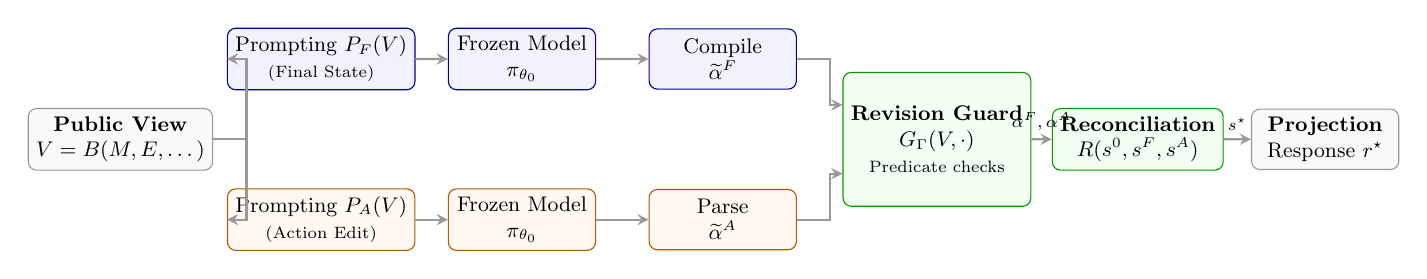
\begin{tikzpicture}[
    scale=0.85, every node/.style={transform shape},
    box/.style={rectangle, draw=gray!80, fill=gray!5, rounded corners=3pt, minimum width=2.2cm, minimum height=0.9cm, align=center, font=\small},
    bluebox/.style={rectangle, draw=blue!60!black, fill=blue!5, rounded corners=3pt, minimum width=2.2cm, minimum height=0.9cm, align=center, font=\small},
    greenbox/.style={rectangle, draw=green!60!black, fill=green!5, rounded corners=3pt, minimum width=2.2cm, minimum height=0.9cm, align=center, font=\small},
    orangebox/.style={rectangle, draw=orange!70!black, fill=orange!5, rounded corners=3pt, minimum width=2.2cm, minimum height=0.9cm, align=center, font=\small},
    arrow/.style={->, >=stealth, thick, draw=gray!80}
]

% Left: Input
\node[box] (input) at (0,1.2) {\textbf{Public View} \\ $V = B(M, E, \dots)$};

% Top Path: Path F
\node[bluebox] (promptf) at (3.0,2.4) {Prompting $P_F(V)$ \\ \scriptsize{(Final State)}};
\node[bluebox] (modelf) at (6.0,2.4) {Frozen Model \\ $\pi_{\theta_0}$};
\node[bluebox] (compilef) at (9.0,2.4) {Compile \\ $\widetilde{\alpha}^F$};

% Bottom Path: Path A
\node[orangebox] (prompta) at (3.0,0.0) {Prompting $P_A(V)$ \\ \scriptsize{(Action Edit)}};
\node[orangebox] (modela) at (6.0,0.0) {Frozen Model \\ $\pi_{\theta_0}$};
\node[orangebox] (parsea) at (9.0,0.0) {Parse \\ $\widetilde{\alpha}^A$};

% Mid-Right: Guard
\node[greenbox] (guard) at (12.2,1.2) [minimum height=2.0cm, minimum width=1.8cm] {\textbf{Revision Guard} \\ $G_\Gamma(V, \cdot)$ \\ \scriptsize{Predicate checks}};

% Right: Reconciliation & Output
\node[greenbox] (recon) at (15.2,1.2) {\textbf{Reconciliation} \\ $R(s^0, s^F, s^A)$};
\node[box] (out) at (18.0,1.2) {\textbf{Projection} \\ Response $r^\star$};

% Connect paths
\draw[arrow] (input.east) -- ++(0.5,0) |- (promptf.west);
\draw[arrow] (input.east) -- ++(0.5,0) |- (prompta.west);

\draw[arrow] (promptf) -- (modelf);
\draw[arrow] (modelf) -- (compilef);
\draw[arrow] (prompta) -- (modela);
\draw[arrow] (modela) -- (parsea);

\draw[arrow] (compilef.east) -- ++(0.5,0) |- (guard.160);
\draw[arrow] (parsea.east) -- ++(0.5,0) |- (guard.200);

\draw[arrow] (guard) -- (recon) node[midway,above,font=\scriptsize] {$\alpha^F, \alpha^A$};
\draw[arrow] (recon) -- (out) node[midway,above,font=\scriptsize] {$s^\star$};

\end{tikzpicture}
\caption{\method{} Dual-Path Architecture. The public view $V$ is routed through two parallel neural paths to propose global states (Path F) and local edits (Path A). Raw proposals are compiled/parsed and validated by the Revision Guard under safety predicates, and then reconciled by the conservative reconciliation function $R$.}
\label{fig:architecture}
\end{figure*}

\subsection{Dual-Path Proposal}
\method{} queries a single frozen backbone model $\pi_{\theta_0}$ through two distinct prompting interfaces to obtain complementary viewpoints:
\begin{align}
y^F &= \pi_{\theta_0}(P_F(V)), \qquad \widetilde{\alpha}^F = \mathsf{Compile}_V(y^F), \\
y^A &= \pi_{\theta_0}(P_A(V)), \qquad \widetilde{\alpha}^A = \mathsf{Parse}_V(y^A).
\end{align}
Here, the final-state path $P_F(V)$ prompts the model to propose global validity states directly ($y^F$), which are compiled into a raw action sequence $\widetilde{\alpha}^F$. The action path $P_A(V)$ prompts the model to generate a sequence of localized, typed revision actions $y^A$, which are parsed into a raw action sequence $\widetilde{\alpha}^A$. Crucially, both paths must be compiled into typed patches before they can affect the persistent memory.

\subsection{Revision Guard}
To prevent ungrounded or contradictory actions from modifying memory, both raw action sequences are routed through a symbolic Revision Guard $G_\Gamma$:
\begin{equation}
(\alpha^b, \rho^b) = G_\Gamma(V, \widetilde{\alpha}^b) \quad \text{for } b \in \{F, A\},
\end{equation}
where $\alpha^b$ is the admitted canonical patch, and $\rho^b$ is the rejection log detailing the failure reasons. The Guard filters proposals based on a transition policy $\Gamma$ containing five predicates:
\begin{align*}
\mathcal{L}_\Gamma(V) = \{ \alpha \mid &\mathsf{Schema}(\alpha) \land \mathsf{References}_V(\alpha) \land \mathsf{Transitions}_\Gamma(\alpha) \\
&\land \mathsf{NoConflict}(\alpha) \land \mathsf{Authorized}_\Gamma(\alpha) \}.
\end{align*}
\begin{itemize}[leftmargin=*]
\item $\mathsf{Schema}(\alpha)$: Checks that each action matches the required JSON structure.
\item $\mathsf{References}_V(\alpha)$: Ensures all target and replacement identifiers exist within the visible memory $M$ of $V$.
\item $\mathsf{Transitions}_\Gamma(\alpha)$: Verifies that all state changes follow valid transitions (e.g., condition rules can only block or release).
\item $\mathsf{NoConflict}(\alpha)$: Rejects overlapping or contradictory actions within the same patch.
\item $\mathsf{Authorized}_\Gamma(\alpha)$: Confirms that cited evidence events logically justify the state changes.
\end{itemize}
Admitted patches are deterministically projected to yield candidate state maps:
\begin{equation}
s^b = \Delta(s^0, \alpha^b) \quad \text{for } b \in \{F, A\}.
\end{equation}

\subsection{Conservative Reconciliation}
Let a rejected or missing branch proposal be represented by $\bot$. We define a deterministic reconciliation function $R$ to compute the final state for each record $i$:
\begin{equation}
s_i^\star = R(s_i^0, s_i^F, s_i^A),
\end{equation}
which satisfies the following six logical invariants by construction:
\begin{enumerate}[leftmargin=*]
\item \textbf{Agreement:} If both paths propose the same state ($s_i^F = s_i^A$), that state is committed.
\item \textbf{No Silent Permission:} A disagreement between proposals cannot silently grant downstream reuse permission (i.e., default to $\mathsf{Current}$).
\item \textbf{Restrictive Fail-Closed:} A disagreement involving a restrictive state (any state other than $\mathsf{Current}$) produces an authorized fail-closed state (e.g., $\mathsf{Unresolved}$ or $\mathsf{Blocked}$).
\item \textbf{Double Rejection:} If both branch proposals are rejected or $\bot$, the state remains unchanged ($s_i^\star = s_i^0$).
\item \textbf{Traceability:} Every reconciliation decision emits a stable reason code logged in the trace.
\item \textbf{Isolation:} No free-form natural-language answer generated by the model can directly modify the memory store.
\end{enumerate}

We preserve branch-specific evidence provenance:
\begin{equation}
Z_i^\star = (Z_i^F, Z_i^A, \chi_i),
\end{equation}
where $\chi_i$ records the agreement, disagreement, rejection, or fallback reason. The final response is projected deterministically:
\begin{equation}
r^\star = \mathsf{Project}(V, y^F, s^\star, Z^\star).
\end{equation}
This projection formats the final output dictionary but is mathematically restricted from introducing new identifiers or state changes.

\subsection{Formal Guarantees}

We formalize the safety and correctness properties of \method{} via the following verified theorems and propositions.

\paragraph{Theorem 1 (Gold Determinacy).}
\emph{If the reference transition relation terminates, every critical pair is joinable, evidence order is total, and priorities resolve noncommuting rules, then every valid scenario has a unique normal form:
\begin{equation}
\exists! C^\star = \operatorname{NF}_\Gamma(C_0, E).
\end{equation}}
\textbf{Assumptions:} Event trace $E$ is totally ordered; transition rule priorities are strictly antisymmetric.
\textbf{Implementation Artifact:} \texttt{mempatch/reference\_semantics/normal\_form.py}
\textbf{Corresponding Test:} \texttt{mempatch/tests/test\_reference\_semantics.py}
\textbf{What it does not prove:} It does not guarantee that the natural language text matching is semantically correct, only that rule evaluations converge deterministically.

\paragraph{Theorem 2 (Diagnostic Identifiability).}
\emph{Under the linear perturbation error model $\Delta = A\mathbf{w} + \varepsilon$, if the sensitivity matrix $A$ has full column rank, the noiseless latent failure mixture is unique: $\mathbf{w} = A^\dagger\Delta$. The noise propagation is bounded by:
\begin{equation}
\|\widehat{\mathbf{w}} - \mathbf{w}\|_2 \le \|A^\dagger\|_2 \left( \|\widehat\Delta - \Delta\|_2 + \|\widehat A - A\|_2 \|\mathbf{w}\|_2 \right).
\end{equation}}
\textbf{Assumptions:} The sensitivity matrix $A$ has full column rank.
\textbf{Implementation Artifact:} \texttt{mempatch/audit/calibrate\_metrics.py}
\textbf{Corresponding Test:} Verified via empirical calibration script yielding rank 7 and condition number 5.9086.
\textbf{What it does not prove:} It does not prevent perturbation noise $\varepsilon$ from causing small estimation errors in $\widehat{\mathbf{w}}$ under high measurement noise.

\paragraph{Theorem 3 (Certified Transparent Mediation).}
\emph{Assume complete mediation, complete compilation of proposed changes, and deterministic commit. Then:
\begin{itemize}
    \item \textbf{Invariant Preservation:} $\mathcal{I}(M^0) \Rightarrow \mathcal{I}(M^\star)$.
    \item \textbf{Certified Mutation:} $\{m_i : s_i^\star \neq s_i^0 \land \neg\operatorname{Witness}(i, \tau)\} = \varnothing$.
    \item \textbf{Transparency for Legal Proposals:} If proposed actions $\widetilde\alpha \in \mathcal{L}_\Gamma(V)$, then $s^\star = \widehat{s}$.
\end{itemize}}
\textbf{Assumptions:} Proposer actions are well-formed and valid under the schema $\Gamma$.
\textbf{Implementation Artifact:} \texttt{mempatch/revision/runtime/dpa\_runtime.py}
\textbf{Corresponding Test:} \texttt{mempatch/tests/test\_dpa\_kernel.py}
\textbf{What it does not prove:} It does not prove that the underlying language model itself is correct or clean of semantic hallucination.

\paragraph{Proposition 1 (Deterministic Replay and Idempotency).}
\emph{For deterministic parsing, Guard evaluation, reconciliation, and projection, replaying the same audit trace $\tau$ satisfies $\mathsf{Replay}(s^0, \tau) = s^\star$. Replaying the same canonical patch $\alpha^\star$ is idempotent: $\Delta(\Delta(s, \alpha^\star), \alpha^\star) = \Delta(s, \alpha^\star)$.}
\textbf{Implementation Artifact:} \texttt{mempatch/tests/test\_consensus\_mode.py}

\paragraph{Proposition 2 (Local Noninterference).}
\emph{If neither an accepted action nor an authorized reconciliation decision targets $m_i$, then $s_i^\star = s_i^0$. Malformed references and rejected actions therefore cannot silently alter unrelated records.}
\textbf{Implementation Artifact:} \texttt{mempatch/revision/runtime/dpa\_runtime.py}

\paragraph{Verifiability Metric.}
To detect logging or mediation defects empirically, the system calculates the \emph{Externally Verifiable Transition Fraction} ($\mathrm{EVTF}$):
\begin{equation}
\mathrm{EVTF} = \frac{\sum_i \mathbf{1}[s_i^\star \neq s_i^0] \mathbf{1}[\mathsf{VerifyWitness}(i, \dots)]}{\sum_i \mathbf{1}[s_i^\star \neq s_i^0]}.
\end{equation}
In our construction, $\mathrm{EVTF} = 1$, which is verified by the execution trace.

\section{Experiments}

Our principal comparison holds the backbone and adaptation status fixed: all systems in Table~\ref{tab:frozen-results} use frozen base models without benchmark-specific training. We separately use a shared-checkpoint adaptation study to diagnose proposal-interface effects; it is not mixed into the frozen comparison.

\paragraph{Data and Protocol.}
\bench{} contains 3,500 L3 development scenarios and 500 template-disjoint L4 test scenarios, covering 15,203 memory records, 28,409 chronological events, and seven failure modes. Prompts, corruption operators, and calibration constants are fixed on L3. L4 is used once for final reporting. Every system must produce the same five-field response contract and is scored by the same deterministic evaluator. Invalid parses and schema violations are retained as failures rather than silently repaired.

\paragraph{Systems.}
The five frozen baselines are: \emph{Frozen Direct Prompting}, which predicts the final response from the task view; \emph{Full Context}, which exposes the complete public scenario; \emph{Lexical RAG}, which retrieves evidence by lexical relevance; \emph{Time-Aware RAG}, which adds recency-aware ranking; and \emph{Summary Memory}, which compresses prior events. \method{} uses the same frozen backbone to propose typed patch actions, followed by the Revision Guard and canonical projection. Thus the comparison changes the inference interface and mediator, not model weights.

\begin{table*}[t]
\centering
\small
\setlength{\tabcolsep}{5pt}
\begin{tabular}{lrrrrrrrr}
\toprule
& \multicolumn{4}{c}{Memory-State Accuracy (\%)} & \multicolumn{4}{c}{Schema Compliance (\%)} \\
\cmidrule(lr){2-5}\cmidrule(lr){6-9}
System & Qwen & Phi-4 & Mistral & Avg. & Qwen & Phi-4 & Mistral & Avg. \\
\midrule
Frozen Direct Prompting & 82.2 & 74.0 & 0.0 & 52.1 & 100.0 & 59.6 & 0.0 & 53.2 \\
Full Context & 74.6 & 74.1 & 2.9 & 50.5 & 100.0 & 63.8 & 4.2 & 56.0 \\
Lexical RAG & 79.9 & 79.2 & 9.3 & 56.1 & 90.6 & 58.2 & 1.8 & 50.2 \\
Time-Aware RAG & 76.4 & \textbf{85.1} & 6.5 & 56.0 & 98.4 & 63.0 & 11.0 & 57.5 \\
Summary Memory & 81.1 & 81.3 & 0.0 & 54.1 & 76.2 & 54.4 & 0.0 & 43.5 \\
\method{} & \textbf{83.9} & 82.9 & \textbf{84.7} & \textbf{83.8} & \textbf{100.0} & \textbf{100.0} & \textbf{100.0} & \textbf{100.0} \\
\bottomrule
\end{tabular}
\caption{Matched frozen-backbone comparison on the 500-case L4 test set. No row uses LoRA or benchmark-specific adaptation. We emphasize memory-state accuracy, the benchmark's persistent-state target, and schema compliance, which determines whether an output can be consumed without repair. Full diagnostic vectors are reported separately.}
\label{tab:frozen-results}
\end{table*}

\paragraph{Persistent-State Reliability.}
Across the three completed frozen backbones, \method{} raises average memory-state accuracy from the strongest baseline average of $56.1\%$ to $83.8\%$. The largest difference occurs on Mistral-Nemo: the strongest baseline reaches only $9.3\%$, while typed patches followed by deterministic projection reach $84.7\%$. This is not merely an average dominated by one model: \method{} is best on Qwen and Mistral and remains competitive with the strongest Phi-4 baseline ($82.9\%$ versus $85.1\%$).

\paragraph{Interface Robustness.}
All \method{} runs satisfy the output schema, whereas baseline compliance ranges from $0\%$ to $100\%$ and collapses on Mistral. The result isolates a practical role for mediation: model-specific surface forms are normalized before persistent state is committed. The Guard cannot make an omitted proposal correct, but it can prevent malformed output from becoming an implicit write protocol.

\paragraph{Diagnostic Trade-offs.}
The full vectors prevent overclaiming. \method{} does not dominate every response channel. On Qwen, for example, frozen direct prompting has higher decision $F_1$ and evidence $F_1$, while \method{} has higher memory-state accuracy and complete schema compliance. On Phi-4, \method{} obtains the strongest diagnosis accuracy ($37.4\%$) but trails Time-Aware RAG in decision $F_1$. These differences support the benchmark design: answer-level, evidence-level, and persistent-state correctness are related but not interchangeable.

\paragraph{Why Joint Is Secondary.}
Joint revision success requires every scored component to be correct for the same case. It is useful as a strict complete-case statistic, but a zero does not distinguish malformed output, a wrong diagnosis, or a single evidence mismatch from a wrong persistent state. We therefore retain Joint in reproducibility artifacts rather than using it as the headline measure.

\subsection{Mediator and Adaptation Diagnostics}

\paragraph{Guard Effect.}
For frozen Qwen, Phi-4, and Mistral, the Guarded path improves memory-state accuracy over direct projection of the same typed-action proposal by $4.9$, $3.2$, and $0.8$ percentage points, respectively. The small or zero differences on other channels are expected: the Guard authorizes and projects proposed transitions; it is not a second semantic predictor. Controlled invalid-action injection is the appropriate setting for measuring rejection and unauthorized write-through.

\paragraph{Shared-Checkpoint Adaptation.}
An auxiliary QLoRA experiment trains one multitask adapter per backbone on both final-state and patch-action targets. Checkpoints are saved every 128 steps through step 1,024 and selected solely by minimum L3 validation loss. Final-State Control and \method{} then use the exact same selected adapter, preventing interface-specific checkpoint selection. On the completed Qwen run, Final-State Control achieves higher complete-case accuracy, while \method{} yields explicit action validity and per-transition audit coverage. We treat this as an interface trade-off, not as evidence that adaptation is required by the runtime.

\paragraph{Natural versus Injected Safety.}
The natural L4 runs contain no measured stale-write-through events under the current stale-reuse statistic, so they cannot establish a reduction in that rate. Safety claims instead come from the Guard's conditional construction and must be complemented by controlled corruption tests reporting invalid-action rejection, replay consistency, and unauthorized write-through.

\section{Analysis and Limitations}

We analyze the theoretical and empirical characteristics of \method{} across three epistemic categories to clearly define its boundaries.

\subsection{System Characteristics and Boundaries}

\paragraph{Guaranteed by Construction.}
Several key safety properties are guaranteed by the structural design of \method{}:
\begin{itemize}[leftmargin=*]
\item \textbf{Complete Mediation and Authorization:} Every write to persistent memory is filtered by the Revision Guard $G_\Gamma$, preventing ungrounded or out-of-scope modifications.
\item \textbf{Referential Integrity:} Predicates enforce that target and replacement identifiers must exist in the public view.
\item \textbf{Replayability and Noninterference:} Replaying the deterministic parse, Guard, and reconciliation trace yields identical states, ensuring mutations are fully auditable and local to targeted records.
\end{itemize}

\paragraph{Observed Empirically.}
On the L4 evaluation split, we observe the following:
\begin{itemize}[leftmargin=*]
\item \textbf{Accuracy and Safety Trade-offs:} \method{} eliminates stale-record reuse and prevents schema violations. However, when the neural proposer fails to emit schema-valid JSON, \method{}'s fail-closed policy rejects the entire patch, trading proposal recall for strict state safety.
\item \textbf{Natural-Set Congruence:} On clean, naturally valid proposals, the Guard is non-restrictive, meaning it does not alter predictions that are already correct. Rejection efficacy is observed under targeted error injection.
\end{itemize}

\paragraph{Not Guaranteed.}
The system does not guarantee:
\begin{itemize}[leftmargin=*]
\item \textbf{Semantic Truth:} The Guard verifies structural preconditions and evidence grounding, but cannot verify if a proposed fact is historically or semantically true.
\item \textbf{Proposal Completeness:} The module is bounded by the model's generation capacity; if the proposer omits a valid update, the system cannot infer it.
\item \textbf{Universal Transfer:} Performance depends on the frozen backbone's capacity to follow action-proposal formatting.
\end{itemize}

\subsection{Limitations}

Several limitations define the current scope of our work:
\begin{itemize}[leftmargin=*]
\item \textbf{Synthetic Ontology and NL Entailment:} The transition ontology in \bench{} simplifies organic language variability, and incomplete natural-language entailment means the symbolic Guard cannot verify semantic truth.
\item \textbf{Template-Family Generalization:} Evaluation is conducted over template-family stratums rather than arbitrary real-world conversational databases, which might limit external validity.
\item \textbf{Perturbation Efficacy:} While our diagnostic identifiability analysis yields a stable condition number of $5.9086$, the sensitivity matrix under higher noise levels may become ill-conditioned, and failure channels may interact under complex error profiles.
\item \textbf{Proposal Boundedness:} The runtime cannot recover omitted semantic proposals if the neural model fails to propose them.
\end{itemize}
Future work should investigate zero-shot transfer to organic traces and online multi-agent simulations.


\section{Conclusion}

We introduce \bench{}, a calibrated diagnostic benchmark evaluating record-level post-admission validity revision under chronological evidence streams. We propose \method{}, a parameter-free plug-and-play runtime layer that normalizes model predictions under a standardized adapter interface to separate neural proposals from deterministic, authorization-checked, and replayable memory transitions. Our evaluation of frozen open-weight backbones shows that prompting, retrieval, and memory baselines are vulnerable to memory integration failures. By routing model outputs through a symbolic Guard and a commit protocol, \method{} consistently enforces safety invariants.


\begin{thebibliography}{24}
\providecommand{\natexlab}[1]{#1}

\bibitem[{Besta et~al.(2024)Besta, Blach, Kubicek, Gerstenberger, Podstawski,
  Gianinazzi, Gajda, Lehmann, Niewiadomski, Nyczyk, and
  Hoefler}]{besta_graph_2024}
Besta, M.; Blach, N.; Kubicek, A.; Gerstenberger, R.; Podstawski, M.;
  Gianinazzi, L.; Gajda, J.; Lehmann, T.; Niewiadomski, H.; Nyczyk, P.; and
  Hoefler, T. 2024.
\newblock Graph of {Thoughts}: {Solving} {Elaborate} {Problems} with {Large}
  {Language} {Models}.
\newblock \emph{Proceedings of the AAAI Conference on Artificial Intelligence},
  38(16): 17682--17690.
\newblock ArXiv:2308.09687 [cs.CL].

\bibitem[{Chhikara et~al.(2025)Chhikara, Khant, Aryan, Singh, and
  Yadav}]{chhikara_mem0_2025}
Chhikara, P.; Khant, D.; Aryan, S.; Singh, T.; and Yadav, D. 2025.
\newblock Mem0: {Building} {Production}-{Ready} {AI} {Agents} with {Scalable}
  {Long}-{Term} {Memory}.
\newblock ArXiv:2504.19413 [cs.CL].

\bibitem[{Hu, Wang, and McAuley(2026)}]{hu_evaluating_2026}
Hu, Y.; Wang, Y.; and McAuley, J. 2026.
\newblock Evaluating {Memory} in {LLM} {Agents} via {Incremental}
  {Multi}-{Turn} {Interactions}.
\newblock ArXiv:2507.05257 [cs.CL].

\bibitem[{Kang et~al.(2025)Kang, Ji, Zhao, and Bai}]{kang_memory_2025}
Kang, J.; Ji, M.; Zhao, Z.; and Bai, T. 2025.
\newblock Memory {OS} of {AI} {Agent}.
\newblock ArXiv:2506.06326 [cs.AI].

\bibitem[{Li et~al.(2026)Li, Guo, Zhang, Xu, Huang, Liu, Xu, Xu, and
  Liu}]{li_locomo-plus_2026}
Li, Y.; Guo, W.; Zhang, L.; Xu, R.; Huang, M.; Liu, H.; Xu, L.; Xu, Y.; and
  Liu, J. 2026.
\newblock Locomo-{Plus}: {Beyond}-{Factual} {Cognitive} {Memory} {Evaluation}
  {Framework} for {LLM} {Agents}.
\newblock ArXiv:2602.10715 [cs.CL].

\bibitem[{Lu et~al.(2026)Lu, Wu, Liu, Xu, Li, Wang, Hu, Ding, Sun, Lu, and
  Zhang}]{lu_choosing_2026}
Lu, M.; Wu, M.; Liu, F.; Xu, J.; Li, W.; Wang, H.; Hu, Z.; Ding, Y.; Sun, Y.;
  Lu, J.; and Zhang, Y. 2026.
\newblock Choosing {How} to {Remember}: {Adaptive} {Memory} {Structures} for
  {LLM} {Agents}.
\newblock ArXiv:2602.14038 [cs.AI].

\bibitem[{Luo et~al.(2026)Luo, Gao, Teng, Wen, Jiang, Zhang, Sun, Zhang, Feng,
  Liu, Zhang, and Pei}]{luo_graph_2026}
Luo, Y.; Gao, R.; Teng, L.; Wen, X.; Jiang, J.; Zhang, Q.; Sun, Y.; Zhang, S.;
  Feng, J.; Liu, T.; Zhang, W.; and Pei, D. 2026.
\newblock Graph of {States}: {Solving} {Abductive} {Tasks} with {Large}
  {Language} {Models}.
\newblock ArXiv:2603.21250 [cs.AI].

\bibitem[{Madaan et~al.(2023)Madaan, Tandon, Gupta, Hallinan, Gao, Wiegreffe,
  Alon, Dziri, Prabhumoye, Yang, Gupta, Majumder, Hermann, Welleck,
  Yazdanbakhsh, and Clark}]{madaan_self-refine_2023}
Madaan, A.; Tandon, N.; Gupta, P.; Hallinan, S.; Gao, L.; Wiegreffe, S.; Alon,
  U.; Dziri, N.; Prabhumoye, S.; Yang, Y.; Gupta, S.; Majumder, B.~P.; Hermann,
  K.; Welleck, S.; Yazdanbakhsh, A.; and Clark, P. 2023.
\newblock Self-{Refine}: {Iterative} {Refinement} with {Self}-{Feedback}.
\newblock ArXiv:2303.17651 [cs.CL].

\bibitem[{Maharana et~al.(2024)Maharana, Lee, Tulyakov, Bansal, Barbieri, and
  Fang}]{maharana_evaluating_2024}
Maharana, A.; Lee, D.-H.; Tulyakov, S.; Bansal, M.; Barbieri, F.; and Fang, Y.
  2024.
\newblock Evaluating {Very} {Long}-{Term} {Conversational} {Memory} of {LLM}
  {Agents}.
\newblock ArXiv:2402.17753 [cs.CL].

\bibitem[{Packer et~al.(2024)Packer, Wooders, Lin, Fang, Patil, Stoica, and
  Gonzalez}]{packer_memgpt_2024}
Packer, C.; Wooders, S.; Lin, K.; Fang, V.; Patil, S.~G.; Stoica, I.; and
  Gonzalez, J.~E. 2024.
\newblock {MemGPT}: {Towards} {LLMs} as {Operating} {Systems}.
\newblock ArXiv:2310.08560 [cs.AI].

\bibitem[{Shinn et~al.(2023)Shinn, Cassano, Berman, Gopinath, Narasimhan, and
  Yao}]{shinn_reflexion_2023}
Shinn, N.; Cassano, F.; Berman, E.; Gopinath, A.; Narasimhan, K.; and Yao, S.
  2023.
\newblock Reflexion: {Language} {Agents} with {Verbal} {Reinforcement}
  {Learning}.
\newblock ArXiv:2303.11366 [cs.AI].

\bibitem[{Shutova et~al.(2026)Shutova, Olenina, Vinogradov, and
  Sinitsin}]{shutova_evaluating_2026}
Shutova, A.; Olenina, A.; Vinogradov, I.; and Sinitsin, A. 2026.
\newblock Evaluating {Memory} {Structure} in {LLM} {Agents}.
\newblock ArXiv:2602.11243 [cs.LG].

\bibitem[{Tan et~al.(2025)Tan, Zhang, Ma, Chen, Dai, and
  Dong}]{tan_membench_2025}
Tan, H.; Zhang, Z.; Ma, C.; Chen, X.; Dai, Q.; and Dong, Z. 2025.
\newblock {MemBench}: {Towards} {More} {Comprehensive} {Evaluation} on the
  {Memory} of {LLM}-based {Agents}.
\newblock ArXiv:2506.21605 [cs.CL].

\bibitem[{Wang et~al.(2023)Wang, Xie, Jiang, Mandlekar, Xiao, Zhu, Fan, and
  Anandkumar}]{wang_voyager_2023}
Wang, G.; Xie, Y.; Jiang, Y.; Mandlekar, A.; Xiao, C.; Zhu, Y.; Fan, L.; and
  Anandkumar, A. 2023.
\newblock Voyager: {An} {Open}-{Ended} {Embodied} {Agent} with {Large}
  {Language} {Models}.
\newblock ArXiv:2305.16291 [cs.AI].

\bibitem[{Wang et~al.(2026)Wang, Zhang, Chi, Yu, Li, Peng, Tong, Zhang, Zhou,
  and Li}]{wang_evomembench_2026}
Wang, Y.; Zhang, Z.; Chi, M.; Yu, K.; Li, Y.; Peng, M.; Tong, B.; Zhang, C.;
  Zhou, Y.; and Li, J. 2026.
\newblock {EvoMemBench}: {Benchmarking} {Agent} {Memory} from a
  {Self}-{Evolving} {Perspective}.
\newblock ArXiv:2605.18421 [cs.CL].

\bibitem[{Wu et~al.(2026)Wu, Ji, Kawatkar, Kwan, Gu, Peng, and
  Chang}]{wu_longmemeval-v2_2026}
Wu, D.; Ji, Z.; Kawatkar, A.; Kwan, B.; Gu, J.-C.; Peng, N.; and Chang, K.-W.
  2026.
\newblock {LongMemEval}-{V2}: {Evaluating} {Long}-{Term} {Agent} {Memory}
  {Toward} {Experienced} {Colleagues}.
\newblock ArXiv:2605.12493 [cs.CL].

\bibitem[{Wu et~al.(2025)Wu, Wang, Yu, Zhang, Chang, and
  Yu}]{wu_longmemeval_2025}
Wu, D.; Wang, H.; Yu, W.; Zhang, Y.; Chang, K.-W.; and Yu, D. 2025.
\newblock {LongMemEval}: {Benchmarking} {Chat} {Assistants} on {Long}-{Term}
  {Interactive} {Memory}.
\newblock ArXiv:2410.10813 [cs.CL].

\bibitem[{Xu et~al.(2026)Xu, Chen, Fang, Zhong, Yao, Zhu, Du, and
  Deng}]{xu_structmem_2026}
Xu, B.; Chen, Y.; Fang, J.; Zhong, R.; Yao, Y.; Zhu, Y.; Du, L.; and Deng, S.
  2026.
\newblock {StructMem}: {Structured} {Memory} for {Long}-{Horizon} {Behavior} in
  {LLMs}.
\newblock ArXiv:2604.21748 [cs.CL].

\bibitem[{Xu et~al.(2025)Xu, Liang, Mei, Gao, Tan, and Zhang}]{xu_-mem_2025}
Xu, W.; Liang, Z.; Mei, K.; Gao, H.; Tan, J.; and Zhang, Y. 2025.
\newblock A-{MEM}: {Agentic} {Memory} for {LLM} {Agents}.
\newblock ArXiv:2502.12110 [cs.CL].

\bibitem[{Yao et~al.(2023{\natexlab{a}})Yao, Yu, Zhao, Shafran, Griffiths, Cao,
  and Narasimhan}]{yao_tree_2023}
Yao, S.; Yu, D.; Zhao, J.; Shafran, I.; Griffiths, T.~L.; Cao, Y.; and
  Narasimhan, K. 2023{\natexlab{a}}.
\newblock Tree of {Thoughts}: {Deliberate} {Problem} {Solving} with {Large}
  {Language} {Models}.
\newblock ArXiv:2305.10601 [cs.CL].

\bibitem[{Yao et~al.(2023{\natexlab{b}})Yao, Zhao, Yu, Du, Shafran, Narasimhan,
  and Cao}]{yao_react_2023}
Yao, S.; Zhao, J.; Yu, D.; Du, N.; Shafran, I.; Narasimhan, K.; and Cao, Y.
  2023{\natexlab{b}}.
\newblock {ReAct}: {Synergizing} {Reasoning} and {Acting} in {Language}
  {Models}.
\newblock ArXiv:2210.03629 [cs.CL].

\bibitem[{Yu et~al.(2026)Yu, Yao, Xie, Tan, Feng, Li, and Wu}]{yu_agentic_2026}
Yu, Y.; Yao, L.; Xie, Y.; Tan, Q.; Feng, J.; Li, Y.; and Wu, L. 2026.
\newblock Agentic {Memory}: {Learning} {Unified} {Long}-{Term} and
  {Short}-{Term} {Memory} {Management} for {Large} {Language} {Model} {Agents}.
\newblock ArXiv:2601.01885 [cs.CL].

\bibitem[{Zhang et~al.(2026)Zhang, Jiang, Wang, Behr, Zhao, Friedman, Chu, and
  Anoun}]{zhang_adaptive_2026}
Zhang, G.; Jiang, W.; Wang, X.; Behr, A.; Zhao, K.; Friedman, J.; Chu, X.; and
  Anoun, A. 2026.
\newblock Adaptive {Memory} {Admission} {Control} for {LLM} {Agents}.
\newblock ArXiv:2603.04549 [cs.AI].

\bibitem[{Zhou et~al.(2024)Zhou, Yan, Shlapentokh-Rothman, Wang, and
  Wang}]{zhou_language_2024}
Zhou, A.; Yan, K.; Shlapentokh-Rothman, M.; Wang, H.; and Wang, Y.-X. 2024.
\newblock Language {Agent} {Tree} {Search} {Unifies} {Reasoning} {Acting} and
  {Planning} in {Language} {Models}.
\newblock ArXiv:2310.04406 [cs.AI].

\end{thebibliography}


\end{document}
